%
% This is the LaTeX template file for lecture notes for CS294-8,
% Computational Biology for Computer Scientists.  When preparing 
% LaTeX notes for this class, please use this template.
%
% To familiarize yourself with this template, the body contains
% some examples of its use.  Look them over.  Then you can
% run LaTeX on this file.  After you have LaTeXed this file then
% you can look over the result either by printing it out with
% dvips or using xdvi.
%
% This template is based on the template for Prof. Sinclair's CS 270.

\documentclass[11pt, twosides]{article}
\usepackage[utf8]{inputenc}
\usepackage{graphicx}
\usepackage{graphics}
\usepackage{amsmath}
\usepackage{amsfonts}
\usepackage{amssymb}
\usepackage{float}
\usepackage{amsthm}
\usepackage[dvipsnames]{xcolor}
\setlength{\oddsidemargin}{0.25 in}
\setlength{\evensidemargin}{-0.25 in}
\setlength{\topmargin}{-0.6 in}
\setlength{\textwidth}{6.5 in}
\setlength{\textheight}{8.5 in}
\setlength{\headsep}{0.75 in}
\setlength{\parindent}{0 in}
\setlength{\parskip}{0.1 in}
%
% The following commands set up the lecnum (lecture number)
% counter and make various numbering schemes work relative
% to the lecture number.
%
\newcounter{lecnum}
\renewcommand{\thepage}{\thelecnum-\arabic{page}}
\renewcommand{\thesection}{\thelecnum.\arabic{section}}
\renewcommand{\theequation}{\thelecnum.\arabic{equation}}
\renewcommand{\thefigure}{\thelecnum.\arabic{figure}}
\renewcommand{\thetable}{\thelecnum.\arabic{table}}

%
% The following macro is used to generate the header.
%
\newcommand{\lecture}[4]{
%   \pagestyle{myheadings}
   \thispagestyle{plain}
   \newpage
   \setcounter{lecnum}{#1}
   \setcounter{page}{1}
   \noindent
   \begin{center}
   \framebox{
      \vbox{\vspace{2mm}
    \hbox to 6.28in { {\bf CS 419M Introduction to Machine Learning
                        \hfill Spring 2021-22} }
       \vspace{4mm}
       \hbox to 6.28in { {\Large \hfill Lecture #1: #2  \hfill} }
       \vspace{2mm}
       \hbox to 6.28in { {\it Lecturer: #3 \hfill Scribe: #4} }
      \vspace{2mm}}
   }
   \end{center}
   \markboth{Lecture #1: #2}{Lecture #1: #2}
}

%
% Convention for citations is authors' initials followed by the year.
% For example, to cite a paper by Leighton and Maggs you would type
% \cite{LM89}, and to cite a paper by Strassen you would type \cite{S69}.
% (To avoid bibliography problems, for now we redefine the \cite command.)
% Also commands that create a suitable format for the reference list.
% \renewcommand{\cite}[1]{[#1]}
% \def\beginrefs{\begin{list}%
%         {[\arabic{equation}]}{\usecounter{equation}
%          \setlength{\leftmargin}{2.0truecm}\setlength{\labelsep}{0.4truecm}%
%          \setlength{\labelwidth}{1.6truecm}}}
% \def\endrefs{\end{list}}
% \def\bibentry#1{\item[\hbox{[#1]}]}

%Use this command for a figure; it puts a figure in wherever you want it.
%usage: \fig{NUMBER}{SPACE-IN-INCHES}{CAPTION}
% \newcommand{\fig}[3]{
% 			\vspace{#2}
% 			\begin{center}
% 			Figure \thelecnum.#1:~#3
% 			\end{center}
% 	}
% Use these for theorems, lemmas, proofs, etc.
\newtheorem{theorem}{Theorem}[lecnum]
\newtheorem{lemma}[theorem]{Lemma}
\newtheorem{proposition}[theorem]{Proposition}
\newtheorem{claim}[theorem]{Claim}
\newtheorem{corollary}[theorem]{Corollary}
\newtheorem{definition}[theorem]{Definition}
% \newenvironment{proof}{{\bf Proof:}}{\hfill\rule{2mm}{2mm}}

% **** IF YOU WANT TO DEFINE ADDITIONAL MACROS FOR YOURSELF, PUT THEM HERE:


\begin{document}
%FILL IN THE RIGHT INFO.
%\lecture{**LECTURE-NUMBER**}{**DATE**}{**LECTURER**}{**SCRIBE**}
\lecture{18}{Introduction to CNN}{Abir De}{Group 18A}{Participants: Mitalee Oza, Parth Dange, Harshit Shrivastava, Varad Mahashabde}
%\lecture{x}{Title}{Abir De}{Group y}

\section{Flow of the notes}
\begin{enumerate}
    \item Convolution Operators
    \item Pooling Operators
    \item Example for a basic CNN
    \item Transfer Learning Model
\end{enumerate}
%__________________________________________
\subsection{Why Convolution?}
We know from the Universal Approximation Theorem that any function can be modelled using Feed-Forward Neural Networks (FFNNs). However the number of parameters can be unmanageably large, requiring a large number of examples and computational resources. However, we can reduce the number of parameters needed by leveraging existing structure in the input. \\
Convolutional Neural Networks (CNNs) are commonly used to process image and video data. They improve on FFNNs by respecting the spatial and temporal structure of the image, where convolution operations combine data in a space-time neighbourhood, and pooling combines data in chunks representing larger blocks of data. This leads to huge reduction in number of parameters.
%__________________________________________
\subsection{Convolution Operators}
A convolution is a linear operation that involves the multiplication of a set of weights with the input.  Element wise multiplication is performed between an array of input data and an array of weights called a filter or a kernel. These can be thought of as neurons most of whose weights are artificially held to be 0.

\begin{table}[H]
  \centering
  \begin{tabular}
    { | c|c|c|c|c | } 
    \hline $x_{1,1}$ & $x_{1,2}$ & $x_{1,3}$ & $x_{1,4}$ & $x_{1,5}$ \\
    \hline $x_{2,1}$ & $x_{2,2}$ & $x_{2,3}$ & $x_{2,4}$ & $x_{2,5}$ \\
    \hline $x_{3,1}$ & $x_{3,2}$ & $x_{3,3}$ & $x_{3,4}$ & $x_{3,5}$ \\
    \hline $x_{4,1}$ & $x_{4,2}$ & $x_{4,3}$ & $x_{4,4}$ & $x_{4,5}$ \\
    \hline $x_{5,1}$ & $x_{5,2}$ & $x_{5,3}$ & $x_{5,4}$ & $x_{5,5}$ \\
    \hline
  \end{tabular}
  \caption{Input to Convolution Layer}
  \label{fig:my_label}
\end{table}
  

\begin{table}[H]
  \centering
  \begin{tabular}
    { | c | c | c | } 
    \hline $w_{1,1}$ & $w_{1,2}$ & $w_{1,3}$ \\
    \hline $w_{2,1}$ & $w_{2,2}$ & $w_{2,3}$ \\
    \hline $w_{3,1}$ & $w_{3,2}$ & $w_{3,3}$ \\
    \hline
  \end{tabular}
  \caption{Kernel}
  \label{fig:my_label}
\end{table}

The operation: You start with a kernel (matrix of weights). Starting at a corner of the input, the kernel is multiplied element wise to the array of an input. The kernel slides over the 2D input performing such element wise operations. The matrix formed by these outputs is the activation map. Each element wise multiplication may further be operated on by a non linearity to form the activation map. 

\begin{figure}[htp]
    \centering
    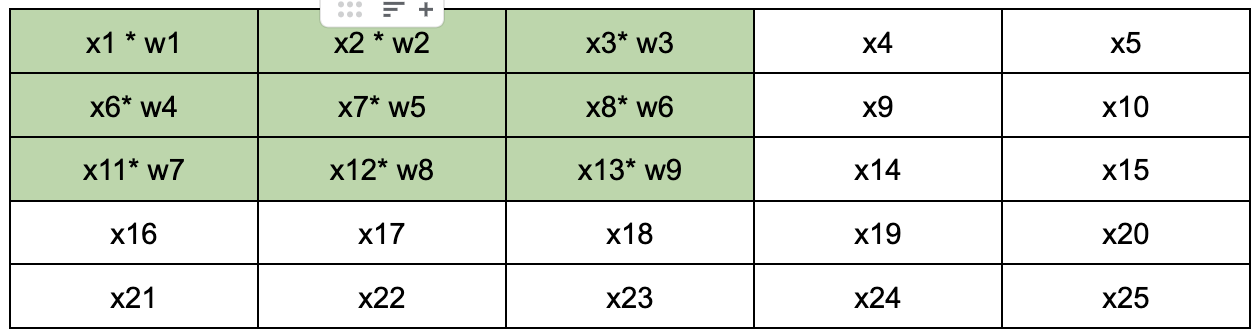
\includegraphics[width=8cm]{first.png}
    \caption{Element-wise multiplication for first convolution output}
    \label{fig:galaxy}
\end{figure}

\begin{align*}
    z_{1,1} &= b &&+ w_{1,1} \cdot x_{1,1} && + w_{1,2} \cdot x_{1,2} && + w_{1,3} \cdot x_{1,3} \\
            &    &&+ w_{2,1} \cdot x_{2,1} && + w_{2,2} \cdot x_{2,2} && + w_{2,3} \cdot x_{2,3} \\
            &    &&+ w_{3,1} \cdot x_{3,1} && + w_{3,2} \cdot x_{3,2} && + w_{3,3} \cdot x_{3,3}
\end{align*}
\begin{equation*}
    o_{1,1} = g(z_{1,1}) \operatorname{ReLU}(z_{1,1})
\end{equation*}

\begin{figure}[htp]
    \centering
    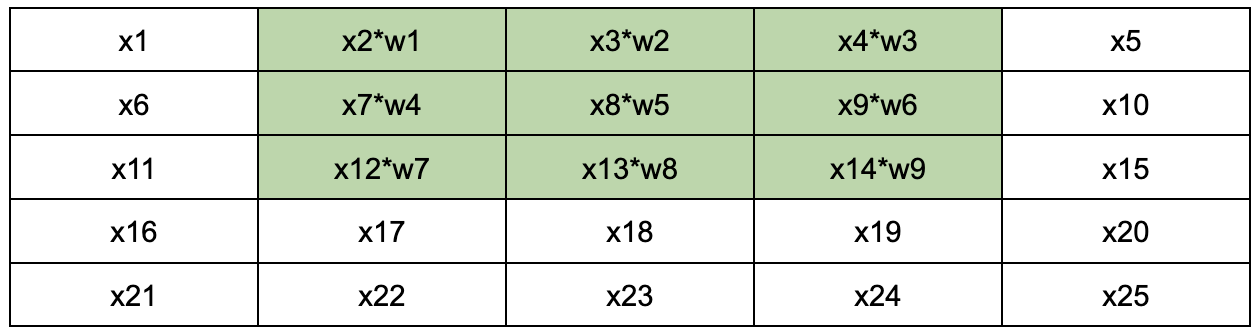
\includegraphics[width=8cm]{second.png}
    \caption{Element-wise multiplication for second convolution output}
    \label{fig:galaxy}
\end{figure}
\begin{align*}
    z_{1,2} &= b &&+ w_{1,1} \cdot x_{1,2} && + w_{1,2} \cdot x_{1,3} && + w_{1,3} \cdot x_{1,4} \\
            &    &&+ w_{2,1} \cdot x_{2,2} && + w_{2,2} \cdot x_{2,3} && + w_{2,3} \cdot x_{2,4} \\
            &    &&+ w_{3,1} \cdot x_{3,2} && + w_{3,2} \cdot x_{3,3} && + w_{3,3} \cdot x_{3,4}
\end{align*}
\begin{equation*}
    o_{1,2} = g(z_{1,2}) = \operatorname{ReLU}(z_{1,2})
\end{equation*}

\begin{table}[H]
  \centering
  \begin{tabular}
    { | c | c | c | } 
    \hline $o_{2,1}$ & $o_{2,2}$ & $o_{2,3}$ \\
    \hline $o_{3,1}$ & $o_{3,2}$ & $o_{3,3}$ \\
    \hline $o_{1,1}$ & $o_{1,2}$ & $o_{1,3}$ \\
    \hline
  \end{tabular}
  \caption{Kernel}
  \label{fig:my_label}
\end{table}

K filters would result in K different activation maps. Further convolution operation can also be used for 3 dimensional images. The filters for this case would be 3 dimensional with the same depth as the image. 
%__________________________________________
\subsection{Pooling Operators}

In pooling, the output from convolution is taken and a filter is applied whose position is such that there is no overlap. The stride will be equal to the length of the filter. Sliding is also used in pooling.

\begin{figure}[H]
    \centering
    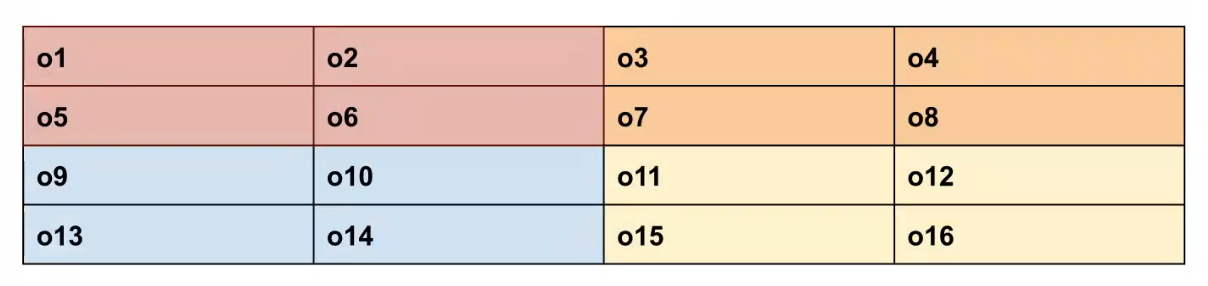
\includegraphics[width=8cm]{filter.png}
    \caption{Filter in pooling}
    \label{fig:galaxy}
\end{figure}

There are two operations in pooling:
\begin{itemize}
    
    \item\textbf{Max pooling}: Each cell will be the maximum of all the operations in the filter
    
\begin{figure}[h]
    \centering
    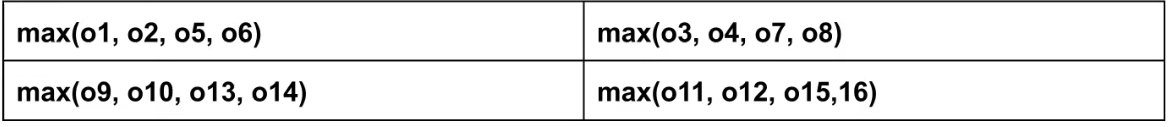
\includegraphics[width=8cm]{max.png}
    \caption{Max pooling}
    \label{fig:galaxy}
\end{figure}

    \item \textbf{Avg pooling} Each cell will be the average of all the operations in the filter
    
\begin{figure}[h]
            \centering
            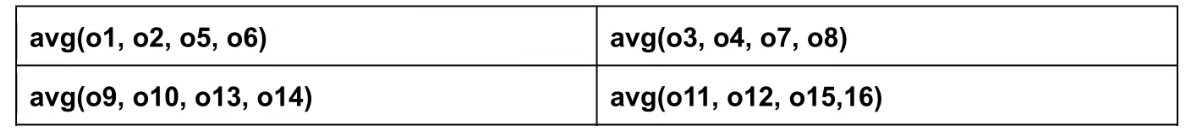
\includegraphics[width=8cm]{avg.png}
            \caption{Average pooling}
\end{figure}
\end{itemize}    

%__________________________________________
\subsection{Example for a Basic CNN}
Let us consider a basic  CNN with the following architecture, where the values in the indices represent the relevant tensor dimensions of the filter.
\begin{align*}
  \text{Input}_{28 \times 28} &\rightarrow \text{Convolution}_{16}^{3\times3} \rightarrow \text{Pooling}^{2\times 2} \rightarrow \text{Convolution}_{32}^{16,3\times3} \rightarrow \text{Pooling}^{2 \times 2} \\
  &\rightarrow \text{Flatten / Vectorize} \rightarrow \text{FFNN} \rightarrow \text{Output}
\end{align*}
\begin{table}[H]
    \centering
    \begin{tabular}{||c||c|c|c|}
      \hline \hline Layer type and Filter Shape & Input Shape & Output Shape & Parameters \\ [0.5ex]
      \hline Input Image & & $\left(28 \times 28 \right)$ & \\
      \hline \shortstack{\textcolor{BrickRed}{Convolution Layer} with 16 filters of \\ size $3\times3$ and stride=1 $\implies$ Filter size = $ \mathcal{F}_{16}^{3\times 3} $} & $\left(28 \times 28 \right)$ & $\left(16, 26 \times 26 \right) $ & $ 16 \cdot \left( 3 \cdot 3  + 1\right)= 160 $ \\
      \hline \shortstack{\textcolor{Turquoise}{Pooling Layer} with size $2\times2$  \\ and stride=2 on each filter } & $\left(16, 26 \times 26 \right) $ & $\left(16, 13 \times 13 \right) $ & \shortstack{0 (has only \\ hyper-parameters)} \\
      \hline \shortstack{\textcolor{BrickRed}{Convolution Layer} with 32 filters of \\ size $3\times3$ and stride=1 \\ $\implies$ Filter size = $ \mathcal{F}_{32}^{16, 3\times 3} $ } & $\left(16, 13 \times 13 \right) $ & $\left(32, 11 \times 11 \right) $ & \shortstack{$ 32 \cdot \left( 16 \cdot 3 \cdot 3  + 1\right) $ \\ = 4640 }\\
      \hline \shortstack{ \textcolor{Turquoise}{Pooling Layer} with size $2\times2$ \\ and stride=2 on each filter } & $\left(32, 11 \times 11 \right) $ & $\left(32, 5 \times 5 \right) $ & 0  \\
      \hline Flatten/Vectorize  & $\left(32, 5 \times 5 \right) $ & $32 \cdot 5 \cdot 5 = 800$ &  \\
      \hline
    \end{tabular}
    \caption{Shape and Parameter counts of the various layers}
    \label{tab:my_label}
\end{table}
We thus observe that we have obtained 800 outputs from 784 inputs from the initial image. However, the new outputs necessarily respect the spatial structure of the image and contain higher-order information about the image. Thus we can have a much smaller FFNN to produce the final output. The reduction in parameters is much more drastic for inputs with larger dimensions. \\
We also note that some information was lost in the second Pooling step as the image could not be neatly divided into pooling regions. We can pad the input image with a few extra empty rows and columns to avoid this.
%__________________________________________
\subsection{Transfer Learning}

The basic idea behind Transfer Learning is to re-use the learned feature maps of a different model and then fine tune them to the specific model we are trying to develop. This proves advantageous as we utilise these learned feature maps without having to start from scratch by training a large model on a large dataset. 

There are two ways we can use this Pre-trained model:
\begin{itemize}
    \item \textbf{Feature Extraction:} Here we use the representations learnt by the pre-trained model and add a new classifier. This new classifier will be learnt from scratch to repurpose the feature maps learned previously for the dataset. We do not need to re-train the entire model.
    \item \textbf{Fine Tuning:} In this method, we freeze all the base layers of the models except the few at the top. Then we add new classifier layers and train these layers along with the unfrozen top layers of the pre-trained model. This way, the higher-order feature representations can be ``fine-tuned" for our specific task
\end{itemize}
%__________________________________________

\section{Group Details and Individual Contribution}

\begin{itemize}
    \item Mitalee Oza: Convolution Operators
    \item Harshit Shrivastava: Transfer Learning Model
    \item Varad Mahashabde: Example CNN
    \item Parth Dange: Pooling Operators
\end{itemize}
\end{document}





